\documentclass[a4paper,12pt]{article}
\usepackage{mathtools,amsfonts,amssymb,amsmath,bm,commath,multicol}
\usepackage{algorithmicx, tkz-graph, algorithm, fancyhdr, pgfplots}
\usepackage{fancyvrb, amsthm, csquotes, booktabs, rotating}
\usepackage{appendix}
\usepackage[backend=biber, citestyle=authoryear]{biblatex}
\renewcommand*{\nameyeardelim}{\addcomma\space}
\addbibresource{thesis.bib}
\usepackage[noend]{algpseudocode}

\pagestyle{fancy}
\fancyhf{}
\rhead{}
\lhead{ Numerocity Biases and the Perceived Chances of Getting a Job }
\rfoot{\thepage}

\begin{document}

\title{ Numerocity Biases and the Perceived Chances of Getting a Job: Experimental Evidence and Implications for Directed Search }

\author{Nandan Rao}

\maketitle

\begin{abstract}

In the labor market, a clear implication of internet-based job applications is the ability of every worker to apply to more jobs without a corresponding increase in the firms' capacity to interview more workers. In this paper, I consider the interaction between the congestion caused by this imbalance and the search behavior of workers.

I hypothesize, and show preliminary experimental evidence that, statistical biases related to numerocity can affect probabilistic judgement in such a way as to cause misjudgements: faster ``applying'' is shown to potentially lead to suboptimal early ``quitting.''

I use estimations from the experimental evidence to calibrate a slightly extended version of the equilibrium directed search model of \cite{gonzalez2010}. Simulations show that this bias causes a hollowing-out of the middle class from the wage distribution, as high-skill workers who experience rejection direct their search to jobs with lower-than-optimal wages.

\end{abstract}

\section{Introduction}

Imagine a job seeker. They spend their first week looking and applying to jobs, and they submit their application to three different positions, all of which fit the profile of their ``dream job''. The next week comes around and they have not heard back from any of the firms. Should they continue to apply to the same type of job, or should they try to look for a job which might be easier to get?

Now consider an alternate universe, where the same job seekers spends their first week looking and applying to jobs, but now the time it takes to find and apply to each job has gone down, and they submit their application to 15 different positions, all of which still fit the profile of ``dream job''. The next week comes around, and they have not heard back from any of the firms. Should they continue to apply to the same type of job?

This paper considers the way in which job seekers react to the above scenario: a technology change that reduces the cost of applying to jobs.

Recent history is rife with technologies that lower the cost of job searching, from the fax machine to the internet to integrated profile-cum-job-boards such as LinkedIn. Given a reduction of costs, be they time or money, the number of applications sent per job seeker will, ceteris parabis, increase. As interviewing is still relatively unmediated by ``time-saving'' technologies, it is clear that the number of outright rejections the average job-seeker receives must increase along with an increase in the number of applications the average job-seeker sends.

It is worth noting the difference between a technology lowering search costs and a technology lowering application costs. The cost of applying for a job consists of two parts: the cost of searching and the cost of actually sending the application. If one lowers the cost of searching, one would expect better-targeted applications. Lowering the cost of applying, whether through reduced search costs or reduced sending costs, has an additional effect, however, which is independent of the targeting: more applications are sent. I will not consider the effect of better-targeting applications in this paper, focusing instead on one potential effect of the increase in application volume in-and-of-itself.

How should we consider, then, the process of a job-seeker estimating the probability of getting a job, to which they apply? Let us split the process into two parts:

1. The job seeker gathers, throughout their entire life, from family, friends, and school, a whole host of preconceptions about the state of the world and their own employability. They listen to the news, they hear rumors, they observe the experiencce of peers.

2. The job seeker applies to some jobs, and through the process of applying, learns more about the probability of receiving offers from each kind of job and firm to which they apply.

This paper considers only the second part, abtracting away from whatever priors the job seeker has from before, I consider how they update their beliefs through the process of applying.

The hypothesis of this paper is nothing more than ``if you get a lot of rejections when applying for a certain type of job, you think your chances of getting such a job are low.'' This thinking is absolutely correct in relative terms, but very much wrong in absolute terms. I propose that job seekers in the real world often act according to absolute terms, a bias which harms them in the high-numbers game of online interactions.

The paper will proceed as follows: in section 2, I will introduce several theories from decision-theory that could potentially be at-play in this scenario. In section 3, I introduce a laboratory experiment to test the way people react to the scenario, prove the optimal reaction, and analyze the results from participants recruited via Amazon's Mechanical Turk. In section 4, I describe an equilibrium model, a slightly extended version of the directed-search model of \cite{gonzalez2010}, and simulate results with parameters calibrated from the laboratory experiments. Finally, in section 5: conclusions and suggestions for further research.


\section { Judging Probabilities }

Does the way in which we, as humans, perform probabilistic calculations change as the numerocity of the problem increases? Several past results indicate yes:

\subsection{Ratio Bias}

A short family tree: Availability Heuristic (\cite{tversky1973}) begets Norm Theory (\cite{kahneman1986}) begets the Ratio Bias (\cite{miller1989}). Whereas the Availability Heuristic relates to memory, the ratio bias is purely about reported statistics, given in the moment.

The idiomatic ratio bias experiment is as follows: there is a kid who really likes chocolate chip cookies, and thinks (like everyone) that oatmeal-raisin cookies are inferior. The kid goes to the cookie jar where there is 1 (10) chocolate cookie, and 19 (190) oatmeal-raisin cookies and picks one, supposedly without looking (as is the rule in the house). He comes back with a chocolate-chip cookie. Do you think he cheated (and looked)? Respondents answer this question differently based on whether there are 20 cookies or 200 cookies, even though the ratios are the same. Specifically, if there is 1 chocolate chip cookie (out of 20), people think it is more likely that the kid cheated (\cite{miller1989}). Often referred to as \textit{denominator neglect}, there is the sense that we focus on the ``norm'' of the numerator, the size of it, in which 1 is less than 10, and therefore the event seems less likely.

\subsection{Numerocity Heuristic}

The origins of this idea can be traced back to a 1941 experiment showing that a kernel of corn, if divided into four pieces, is a more motivating reward for chickens than a single, undivided kernel (\cite{wolfe1941}). Humans, it turns out, are not so different, and systematically confuse numerocity (number of units) for quantity (actual amount). \cite{pelham1994} develop a framework, referred to as the numerocity heuristic, in which this bias is shown to be especially present when individuals attempt to make judgements while under cognitive load, in which case they fall back on numerocity as a rule-of-thumb for determining quantity. This line of research has been explored extensively in the consumer-behavior literature, where preferences are easily shifted based on a changing of scales (cite cite cite).

Is it plausible that, while deciding on the next job application to send, job seekers use ``number of rejections'' as a heuristic for ``expected value of sending one more application'', not fully taking into consideration the denominator (time spent on each application) while doing so? I propose that this is exactly the case.

\subsection{Learning by Experience}

What about the way in which we judge the probability of rare events? It is worth noting that our context here is decidedly different from the one considered in prospect theory and its derivatives (\cite{kahneman1979}), which concern the judgement of probabilities based on external knowledge, primarily given via descriptions of the events. This distinction between \textit{decisions from description} and \textit{decisions from experience} is made in \cite{hertwig2004}, which gives a good overview of the field as well as decisive experiments that show the way in which decision-makers act differently, even oppositely, based on whether they learned about the probability of an event through trial-and-error or through written description.

Specifically, and opposed to Prospect Theory, learning by experience is shown to cause people to \textit{underweight} the probability of rare events, both positive and negative. Note that this seems to be very much independent of the Availability Heuristic, which cites our ability to pull a representative example from memory (\cite{tversky1973}), as this result holds for experiments in which the participant has, immediately before, experienced both outcomes, and for ones in which they have not.

While this is in-and-of-itself interesting and applicable to this research, \cite{hertwig2004} notes one other curious fact for which no explanation is given: in the cited experiments, users are allowed to ``sample'' from a given one-armed bandit as much as they like in a practice round without any specific end, before ``playing for keeps.'' Participants, it seems, chronically undersampled: they quit practising sometimes before even coming accross the a rare outcome with a very large positive or negative reward, the knowledge of which would potentially change their behavior.

This paper attempts to answer that very question: how do people estimate the probability of an unseen rare event? Do they ``snap'' their estimate to zero after not seeing the outcome in some number of chances, effectively assigning measure zero to events they have not seen?


\section{ An MTurk Experiment }

\subsection{ Experimental Design }

This experiment was designed specifically for MTurk, taking advantage of several specific features of the platform and those who use it:

\begin{enumerate}
\item Task creators can specify the characteristics of those who see and can perform their task. This allows us to target, for example, only professional Turkers with a similar level of experience.
\item Turkers with similar qualifications (number of successfully-completed jobs, country, language, etc.) have access to the same pool of jobs at any given time, and therefore similar opportunity costs.
\item On a daily basis, Turkers must decide which jobs are worth doing and which are not. So much so, that there are review websites\footnote{\url{https://turkerview.com}} set up, specifically so that Turkers can review job posters, and in which they report the calculated hourly wage of the job. As such Turkers have, embedded in their very cultural institutions, a very explicit concept of opportunity costs and hourly wages while performing tasks.
\end{enumerate}

Participants are shown boxes which are played much like slot machines and will randomly ``pay out'' with unknown but fixed probability. The boxes are shown to participants one-at-a-time and the game ends when participants win a box or quit, whichever comes first. Participants are told, however, that they were randomly assigned to one of two groups: in the first, the probability of winning is small, in the second, the probability of winning is zero.

The treatment effect is on the speed of the box roll. Treatment group A can theoretically play a new box about once every 3 seconds. Group B, on the other hand, can only play a new box about once every 12 seconds.

Participants who got lucky and won are excluded from the results. The question is: ``how many losses do you experience before you quit trying?''

\subsection{ Rational Response }

In this game, as in applying to jobs, players have two unknown variables to estimate, both of which affect the probability of winning:

\begin{enumerate}
\item The group the player belongs to (the ``skill'' the applicant has), $a_i, i \in \{L,H\}$.
\item The (unkown) probability of payout, $\gamma$, given that they are in the group $a_H$.
\end{enumerate}
%
Rolls are modelled as Bernouli random variables:
\begin{align*}
k_{n+1} \thicksim Bernouli( p ) \\
p \coloneqq P(a_H | n)P(\gamma | n)
\end{align*}
Clearly, the two variables are not uniquely identifiable without further assumptions. In general, the difference between updating one's beliefs about one's own characteristics versus updating one's beliefs about the ``tightness'' of the labor market is extremely significant. In the scope of this experiment, however, participants' ``personal'' characteristics are given externally, by the experimenter, and it is not in any way personal, permanent, or connected to ego. For this reason, in both this proof and in the empirical bias estimates that we infer from the results, we model the joint estimation problem as one of estimating $p$ with the posterior mean $\hat{P}_n$ after $n$ failures, regardless of how exactly it is done, which allows us to model behavior in this particular situation without making any additional assumptions.

I model the problem as an optimal stopping time problem with a finite horizon in which there is no discounting. Consider, for example, the horizon to be the ``work day'' of the Turker. Quite naturally, the worker cannot consume the wage until after the period is finished, so the utility is considered to be the utility of consumption of the period as-a-whole. In this framework, there is also no discounting. The value after playing $n$ rounds is then given by the maximum being the value of continuing to play and the value of quitting.
%
$$
V(n) = \max \left\{ \mathbb{E}V_p(n), V_q(n)  \right\}
$$
%
Where the value of quitting it given by:
%
$$
V_q(n) = u\left( \sum_n^T ct \right)
$$
%
With $c$ is the per-second wage of the outside option and $t$ is the number of seconds per round of play. The expected value of playing is then given in recursive form as:
%
$$
\mathbb{E}V_p(n) = \hat{P}_n u(W + \sum_{n+1}^T ct) + (1 - \hat{P}_n) \mathbb{E}V(n+1)
$$
%
Where $W$ is the prize from winning. The stopping time is thus given by:
$$
\mathbb{E}V_p(n) = u\left( \sum_0^T ct \right)
$$
%
Assume now that there exists some future period, $n+1$, in which it is not optimal to play. With this assumption, we can define the conditions for stopping at time $n$:
%
$$
\mathbb{E}V_p(n) = V_q(n)
$$
Using our assumption about $n+1$ (in which $V(n+1) = V_q(n+1)$), we can rewrite $\mathbb{E}V_p(n)$ as:
\begin{align*}
\mathbb{E}V_p(n) &= \hat{P}_n u(W + \sum_{n+1}^T ct) + (1 - \hat{P}_n)u\left( \sum_{n+1}^T ct \right) \\
\mathbb{E}V_p(n) &= \hat{P}_n \left[   u(W + \sum_{n+1}^T ct) - u\left( \sum_{n+1}^T ct \right) \right]+ u\left( \sum_{n+1}^T ct \right)
\end{align*}
%
Which implies a stopping time of:
$$
\hat{P}_n \left[   u(W + \sum_{n+1}^T ct) - u\left( \sum_{n+1}^T ct \right) \right] = u\left( \sum_n^T ct \right) - u\left( \sum_{n+1}^T ct \right)
$$
%
Letting $u^m_{n}$ denote the marginal utility of some consumption above and beyond $\sum_{n}^T ct$, we can write the stopping time conditions as follows:
$$
\hat{P}_{n} u^m_{n+1}(W) = u^m_{n+1}(ct)
$$

\subsection{ Results }

Summary statistics of the results provided in table \ref{table:descriptive-3}.

What we want to test is whether or there is a difference between how participants in the two treatment groups calculate $\hat{P}_n$, and how that differs from the correct Bayesian estimation. If we knew the opportunity cost of time, $c$, the utility function, and the horizon, we could back out their estimate of the probability:
$$
\hat{P}_{n}  = \frac{u^m_{n+1}(ct)}{u^m_{n+1}(W)}
$$
%
Thus, it might be instructional to assume a functional form for the marginal utility, assume perfect Bayesian probability updating, and then calculate the implied opportunity cost by their measured stopping time. Given a correct assumption of the functional form, and given the null hypothesis of any errors in probability updating to be equal between the treatment groups, we expect the opportunity costs to be equally distributed for both groups.

These estimates are provided in table \ref{table:descriptive-3}, where one can see the results of a Mann Whitney U test between the distribution of costs for both groups. A couple of facts jump out:

\begin{enumerate}
\item The implied opportunity costs are very high: about \$75 per hour for group A and \$50 for group B, assuming the identity utility function (risk neutrality).
\item The implied opportunity costs of the two groups likely come from different distributions.
\end{enumerate}

Given the high implied opportunity cost, we infer that our participants decrease their probability estimate of winning too quickly. This is in accordance with the literature regarding probability estimation of rare events from experience (\cite{hertwig2004}), in which participants underestimate the probability of rare events. Additionally, we can weakly infer from this evidence that the strength of this bias is positively correlated with the numerocity of the problem: if you increase the scale of the problem (by increasing the speed), you worsen the bias.


\section{ An Equilibrium Model }

How can biases of probability judgement affect the labor force on an aggregate level? Specifically, if these biases affect the way a job seeker decides where to search, what effects can they have on unemployment and wage distributions across the labor market?

In order to model such effects, we will need a model with:
%
\begin{enumerate}
\item Agent(s) that direct their search towards specific ``submarkets'' of jobs with different wage characteristics.
\item Agent(s) that do not know the objective probabilities of getting a job in any particular submarket, and must estimate these probabilities through a process of learning by experience.
\item Agent(s) that can experience both rejection and success in searching for jobs, and update their beliefs accordingly.
\end{enumerate}
%
A natural fit is to consider directed search models from the field of search and matching labor market models. Refer to \cite{wright2017} for a survey of directed search models.

There are several models from the directed search literature that attempt to model the effects of multiple applications directly (\cite{albrecht2006}, \cite{galenianos2009}, \cite{wolthoff2017}). These papers primarily focus on characterising the game between firms and workers when workers can receive multiple offers at once and might reject an offer, and firms receive multiple offers at once and must pick one to which they send the offer. While applicable to the larger contextual question of this paper, the focus is very different. This paper focuses on the process of learning an unknown probability of receiving a job, not the process of deciding where to apply once that probability has been estimated.

It is also worth noting that I have not added on-the-job search to the list of requirements. For the purposes of this paper, this serves as a simplifying assumption. It is, however, potentially important to consider the true equilibrium effects of this bias and the way people search for jobs and update their beliefs about their chances in the job market.

\cite{gonzalez2010} offers a unique directed-search equilibrium model that fulfills all of the above requirements, and is the only such model that I am aware of.

\subsection{ Model Specification }

Please refer to \cite{gonzalez2010} for full specification of the model.

For our purposes, I focus here on the the updating of beliefs. In the baseline model, workers are heterogeneous and endowed with skill $a_i, i \in \{ H, L \}$, and the exogenous distribution of the skills is known to everybody. All workers start with homogeneous beliefs about their skill (the expected value given the exogenous distribution). They perform a dynamic programming exercise to determine the submarket with the highest expected value, and apply. Workers are matched to a job with probability $ax$, where $x$ is simply the submarket, continuously valued. After each ``round,'' workers update their beliefs via Bayesian updating, leading to an equilibrium tree of all possible beliefs and submarkets that are ``active.'' From this equilibrium tree, we extract the values of employment and unemployment.

It is easily shown that given the above assumptions, the posterior updates are:
%
\begin{align*}
  \phi(\mu) &\equiv  a_H + a_L - a_Ha_L/\mu \\
  H(x, \mu) &\equiv a_H - (a_H - \mu)(1 - xa_L)/(1 - x\mu)
\end{align*}
%
Where $\phi$ represents an update after a successful match, and $H$ an update after a rejection. The posterior probability after $n$ rejections, $\hat{P}_n$, is then quite naturally defined within this model as the functional composition of $n$ posterior updates, such that the belief after 2 rejections is given by:
$$
\hat{P}_2 \equiv H(g(H(g(\mu_0), \mu_0)), H(g(\mu_0),\mu_o))
$$
Thus, the posterior update after $n$ rejections, taking $\mu_0$ as given, takes the following form:
%
$$
\hat{P}(n): \mathbb{N} \rightarrow \mathbb{R}
$$
%
I extend the model to incorporate a very simple and flexible bias parameter:
%
$$
\hat{P}^{mod}(n) \equiv \hat{P} (n(1 + \epsilon))
$$
This bias linearly increases the number of rejections, such that a job seeker will react after 1 rejection as though they had received $1 + \epsilon$ rejections.

While flexible, this bias parameter does not fit into the functional form of our posterior estimate as defined above, only being defined on the natural numbers and therefore not defined on $N(1 + \epsilon), \epsilon \in \mathbb{R}$.

To solve this problem, I take a first-order approximation of $\hat{P}^{mod}_n$, using finite differences from the surrounding naturals to numerically approximate the first derivative, thus defining $\hat{P}^{mod}_n: \mathbb{R} \rightarrow \mathbb{R}$ in the model space.

\subsection{ Calibration }

I use the empirical results from the second experiment to estimate the bias parameter, $\epsilon$, the only parameter I will explicitly calibrate.

A priori, we do not know the opportunity cost of time of each of the workers, but we can use the assumptions that A) they come from the same distribution and B) the distribution is limited in how spread we believe it is, we can estimate the opportunity cost for each participant as:
$$
c_i \sim \text{DoubleExponential}(\mu^c, \sigma^c)
$$
Where $\mu^c$ and $\sigma^c$ are hyperparameters estimated using TurkerView, a website where Turkers review tasks and task-creators, including posting the calculated hourly wage of each task. 15 participants from the experiment left reviews on TurkerView, and from each of those 15 participants, I scraped the most recent 50 reviews of other tasks they had completed. As such, I assembled a small sampled of about 700 hourly wages. The hyperparameters were then estimated by minimizing the KL-divergence between the fitted truncated double exponential distribution and the scraped wages.

We then estimate a bias parameter for each individual::
\begin{align*}
  \epsilon_i \sim \text{Normal}(\mu^{\epsilon}_g, \sigma^{\epsilon}_g)
\end{align*}
Where treatment parameters $\mu^{\epsilon}_g$ and $\sigma^{\epsilon}_g$ are learned hierarchically for each treatment group, $g$. I use an uninformative half-Cauchy prior on the median and weak inverse-gamma prior on the variance. Exact specifications of all the model are available in the online supplementary materials and code.

The probability estimation is given by:
\begin{align*}
  p_{i} = \frac{1}{1 + N_i(1 + \epsilon_g)}
\end{align*}
Where $p_{i,g}$ indicates the posterior mean estimated probability of winning of individual $i$ from group $g$ after $N_i$ rolls. We then ensure the condition:
$$
p_{i,g} u\left( W \right) = u\left( c_it_i \right)
$$
Where $t_i$ is the mean time between each roll measured for participant $i$. Marginal utility is assumed to be linear. For tractability the constraint is softened by assuming:
$$
\frac{p_{i,g}W}{c_it_i} \sim \text{LogNormal}(0, \frac{1}{\delta})
$$
With penalty term $\delta$ chosen to be sufficiently large to ensure the condition. The theoretical model, while close, does not align exactly with the empirical model I have chosen. This is driven by several simple, and common, assumptions in the theoretical model:
%
\begin{enumerate}
\item All applicants know the probability of a successful job application conditional on their skill level.
\item Skill level is a binary discrete variable (``low'' or ``high''), and as such the estimated posterior mean of this variable is a non-linear function of the numbers of rejections (or successes).
\item The probability of getting a job in any given submarket is linear in skill (the probability is given, simply, by $xa$, where $x$ is the submarket and $a$ is the skill level).
\end{enumerate}

The nature of the last two assumptions is that job seekers update their beliefs quickly after the first couple of rejections, and given the discretization of the submarket space into a reasonably small number of submarkets, they quickly end up searching the lowest possible submarket after a few rejections. Because of this quirk of the model, we cannot appropriately add the exact biases that we have estimated: any bias over 1 will cause the same behavior. Thus, we calibrate the model by normalizing the lower bias to 0. In other words:
%
\begin{equation} \label {eq:epsilon-model}
\epsilon^{mod}_{g} = \frac{\epsilon_g - \min(\epsilon_g, \epsilon_{g'})}{\min (\epsilon_g, \epsilon_{g'})}
\end{equation}
%
Where $\epsilon_{g}$ is the empiricallly estimated bias for treatment group $g$, and $g'$ represents the other treatment.

\subsection{ Results }

Figure \ref{fig:posterior-mean-bias} shows the posterior distribution of the two location parameters, $\mu_{\epsilon, g}$, calculated via Hamiltonian MCMC.

It is worth noting that, sampling from this posterior, one can reject the null hypothesis that the mean bias of group B is greater than or equal to group A at a 0.9\% level. This serves as additional evidence that the treatment significantly affects the way participants compute posterior probabilities.

Full model parameters are provided in table \ref{table:model-params}, although these parameters should be considered extremely preliminary, as they were not calibrated specifically for this model. The results of posterior-updating bias on the wage-distribution outcomes, however, seem very robust to the rest of the model's calibration.

Equilibrium consists of a ``tree'' of beliefs generated from ex-ante heterogeneous agents with homogeneous prior beliefs about their own skill, along with the relative amounts of employed and unemployed agents at each ``belief node.'' The tree is binary, and each node has two children: one for the belief that would result from a rejection (given the current belief), and one that would result from a successful application. The beliefs, in turn, imply a submarket and thus a wage for all the employed agents. Only a portion of all the potential submarkets are active at any given time, leading to a very discrete and spiky wage distribution when plotted on a continuous scale, as the wages from the ``non-active'' submarkets are not received by anyone.

Figure \ref{fig:wage-distributions} shows the simulated wage distributions generated by the calibrated equlibrium model with bias parameter calculated as per (\ref{eq:epsilon-model}) using the median posterior values of $\epsilon_g$ as point estimates. I have added a small amount of noise to plot the wage distributions, purely for visualization purposes, but you can still clearly see the modes that correspond to the active submarket wages.

In the zero-bias model one can clearly see three modes that correspond to workers who were rejected zero, one, and two times respectively, before getting their first job. In the biased model, this middle mode disappears as workers are more pessimistic after their first rejection, and thus apply to lower-wage jobs.

While this is a stylized model, the results are nonetheless telling: greater bias leads to an erosion of the middle class. Both high- and low-skill workers who get unlucky in their initial applications end up in lower-wage jobs then they would with a less biased estimate of their chances in the market.

\section{ Conclusions and Future Research }

I have shown experimental evidence that participants in a probabilistic game estimate the probability of winning, or relate to their opportunity costs, differently based on the speed of game play. This result is not consistent with expected utility and rationality, but it is consistent with several well-studied biases in probability estimation and learning by experience. These biases can cause job seekers to react suboptimally to technologies that allow them to apply to jobs more quickly, causing them to underestimate their chances in the job market.

The effects of this underestimating in the real world are not known, but given the assumptions of the directed-search model of \cite{gonzalez2010}, it leads to a hollowing out of middle-class jobs as workers get easily discouraged in their search.

Understanding how individuals direct their job search is crucial if we want to model the labor market and the impact of policies on its efficiency. I have argued that job search is, at its core, a process in which individuals must necessarily make judgements about the probabilities of favorable outcomes to different actions.

Learning by experience is one way in which individuals estimate these probabilities and this paper has focused on enumerating and testing some statistical biases related to learning by experience. In the experiments, and in the cited literature, I have only considered these biases in ``impersonal'' contexts. If one judges the probability of winning a ``game'' to be low, this has nothing to do with their own value or self-worth as an individual. If one judges the probability of getting a job to be low, this a lot to do with their own value and self-worth as individuals!

A simple extension and logical next step would therefore be to understand how learning-by-experience biases change when one is estimating something that might reflect positively or negatively on one's own self image. In the words of Anthony Greenwald (1980):

\begin{displayquote}
One of the best established findings in social psychology is that people perceive themselves readily as the origin of good effects and reluctantly as the origin of ill effects...
\end{displayquote}

It must also be considered that learning by experience is not the only, and may not even be the primary, way in which individuals estimate the probability of getting a job. Clearly, people do not apply to every single job they would enjoy doing: they know a prior that they are ``not qualified'' to do certain jobs, akin to estimating the probability of success to essentially zero in those contexts. This estimation involves preconceptions about the world that not only might affect the way in which people direct their search much more than learning by experience, but also might affect the way in which people learn by experience.

This opens the question: how does public and private discourse affect the way in which people search for jobs? It is not hard to imagine that repeated exposure to negative discussions about the state of the economy and a high unemployment rate might come quickly to one's mind after a few rejections, even if it one felt quite confident beforehand.

Additionally, I believe it is important to note that all of these affects might not only impact the directed search itself, but also the entire perception of bargaining power held by the majority of workers. If one underestimates the probability of getting a job, is one less likely to bargain for a higher wage, form a union, or petition for a raise after the first year? In short, is it possible that a major change in the perceived bargaining power of workers can be caused by something as simple as a theoretically benevolent technological change that has the unfortunate side effect of increasing the absolute number of rejections for the majority of job seekers.


\printbibliography

\newpage

\begin{appendices}

\section{Tables \& Figures}
\label{appendix:graphs}


\begin{sidewaystable}
  \caption{Summary Statistics for Experiment 2}
  \label{table:descriptive-3}
  \begin{center}
    \begin{tabular}{lcccccccc}
      \hline
      & Group & N & t &  Rolls  &  Time played & c ($\rho = 2$) & c ($\rho = 1$) & c ($\rho = 0$)\\
      \hline
      \hline \\ [-1.8ex]
      Median &         a & 29 &          4 &    54 &  240 &        0.0204 &                 0.0209 &                    2.1368  \\
      &         b & 28 &         15 &    18 &  311 &               0.0138 &                 0.0141 &                    1.4448  \\
      Mean &         a & 29 &          5 &    77 &  374 &          0.0348 &                 0.0356 &                    3.6450  \\
       &         b & 28 &         17 &    24 &  400 &              0.0200 &                 0.0204 &                    2.0875  \\
      \hline \\ [-1.8ex]
      MW p-val & & & & & & 0.084 & 0.084 & 0.078 \\
      \hline \\ [-1.8ex]
      \multicolumn{8}{l}{\textit{Where $t$ is roll time and $c$ is opportunity cost in cents per second and $\rho$ risk aversion in CRRA function}} \\
    \end{tabular}
  \end{center}
\end{sidewaystable}

\begin{table}
  \caption{Model Parameters}
  \label{table:model-params}
  \begin{center}
    \begin{tabular}{lcc}
      \hline
      & Group B & Group A  \\
      \hline
      \hline
      B         &    0.70 &    0.70  \\
      aH        &    1.00 &    1.00  \\
      aL        &    0.05 &    0.05  \\
      b         &    0.03 &    0.03  \\
      bias      &    0.00 &    0.55  \\
      c         &    0.05 &    0.05  \\
      delta     &    0.01 &    0.01  \\
      precision &    0.01 &    0.01  \\
      r         &    0.04 &    0.04  \\
      sigma     &    0.10 &    0.10  \\
      y         &    0.11 &    0.11  \\
      \hline
    \end{tabular}
  \end{center}
\end{table}

\begin{figure}[h]
    \centering
    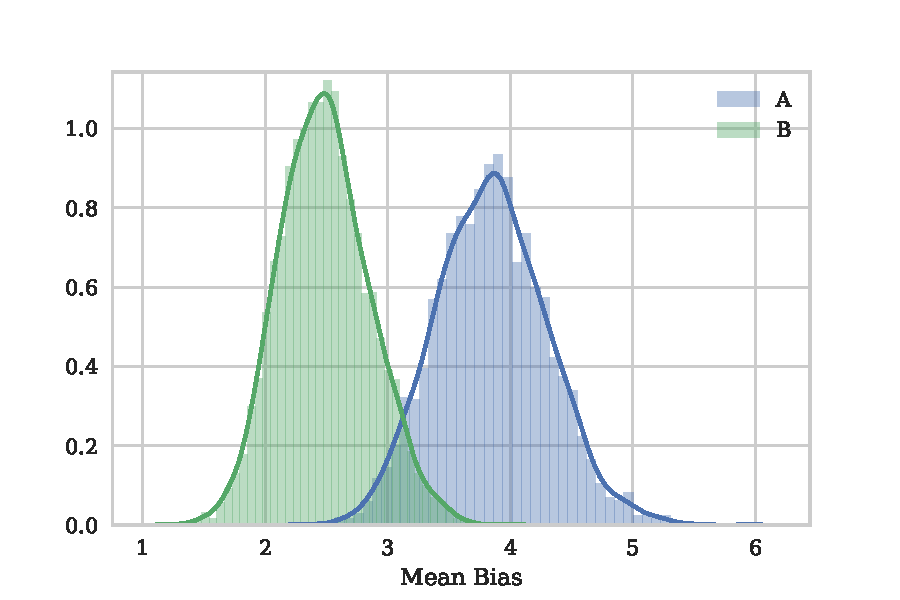
\includegraphics[width=0.8\textwidth]{../experiments/mean-bias}
    \caption{Posterior distribution for mean bias parameter}
    \label{fig:posterior-mean-bias}
\end{figure}

\begin{figure}[h]
    \centering
    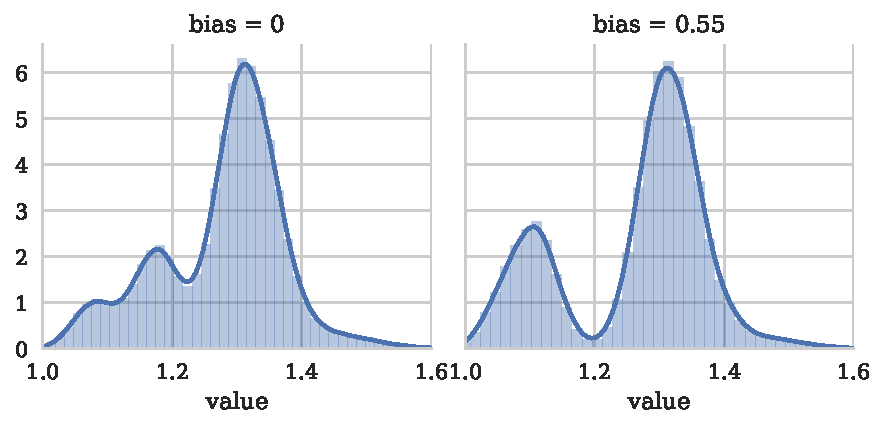
\includegraphics[width=0.8\textwidth]{../equilibrium/wage-distributions}
    \caption{Equilibrium wage distributions with estimated bias differential}
    \label{fig:wage-distributions}
\end{figure}

\newpage

\end{appendices}
\end{document}